\documentclass[conference]{IEEEtran}
\IEEEoverridecommandlockouts
% The preceding line is only needed to identify funding in the first footnote. If that is unneeded, please comment it out.
\usepackage[T1]{fontenc}
\usepackage[utf8]{inputenc}
\usepackage[spanish]{babel}	
\usepackage{amsmath,amssymb,amsfonts}
\usepackage{cite}
%\usepackage{algorithmic}
\usepackage{graphicx}
\usepackage{balance}
\usepackage{textcomp}
\def\BibTeX{{\rm B\kern-.05em{\sc i\kern-.025em b}\kern-.08em
    T\kern-.1667em\lower.7ex\hbox{E}\kern-.125emX}}
\begin{document}

\title{Modelo de Programación MapReduce para Hadoop}

\author{\IEEEauthorblockN{1\textsuperscript{st} Francisco Sans}
\IEEEauthorblockA{\textit{Centro de Comptuación Gráfica} \\
\textit{Universidad Central de Venezuela}\\
Caracas, Venezuela \\
francisco.sans@ciens.ucv.ve}
}

\maketitle

\begin{abstract}
El volumen de datos producidos que deben ser almacenados y procesados ha aumentado de manera considerable en los últimos tiempos.
Además, recientemente ha surgido la necesidad de poder analizarlos y obtener información significativa a partir de estos datos, siendo uno de los grandes retos de nuestra era.
Por ello, han surgido herramientas como Hadoop, las cuales de manera eficiente permiten almacenar y realizar operaciones sobre grandes cantidades de datos.
Uno de los aspectos más relevantes de esta herramienta es el uso del modelo de programación MapReduce, el cual permite el procesamiento eficiente de los datos.
Este trabajo tiene como objetivo servir como una introducción teórica a este modelo de programación y su implementación en Hadoop, considerando sus ventajas y sus limitaciones.
\end{abstract}



\begin{IEEEkeywords}
Haddop, MapReduce, Modelo de Programación
\end{IEEEkeywords}



\section{Introduction}
\label{intro}

Actualmente se produce de manera diaria grandes volúmenes de datos que sobrepasan las capacidades de almacenamiento y de procesamiento de una computadora convencional~\cite{Holmes12}.
Recientemente, el campo de estudio de Big Data trata de solventar los problemas de cómo almacenar y trabajar con volúmenes de datos excesivamente grandes, además de buscar soluciones de como analizarlos y obtener información significativa a partir de ellos.

Una de las herramientas más utilizadas en Big Data es Hadoop~\cite{Hadoop}.
Hadoop es un sistema distribuido que ofrece una manera de paralelizar y ejecutar programas en grandes clusters de computadoras.
Posee una arquitectura maestro/esclavo que contiene el Hadoop Distributed File System (HDFS~\cite{HDFS10}) para el almacenamiento de datos (basado en el sistema de archivos de Google GSF~\cite{GoogleFS03}) y el \textit{framework} MapReduce~\cite{MapReduce04}\cite{MapReduceII08} para realizar cómputos.
Entre las principales cualidades de Hadoop es el particionamiento de la data y la computación paralela de grandes volúmenes de datos.
Ambas cualidades escalan con la adición de nodos al cluster de Hadoop, y pueden alcanzar un volumen de datos de petabytes en clusters con muchos nodos.



En este trabajo se hará una breve introducción al uso del modelo de programación MapReduce y su uso en Hadoop, y se encuentra organizado de la siguiente manera: 
en la Sección~\ref{map} se expondrán los conceptos básicos de este modelo de programación y algunos ejemplos de soluciones a problemas resueltos con este modelo;
la Sección~\ref{hadoop} describirá como este modelo es implementado en los diferentes componentes de Hadoop;
la Sección~\ref{limits} explicará algunas de las limitaciones encontradas en el uso del MapReduce; y 
finalmente, la Sección~\ref{conclu} mostrará las conclusiones con algunas ideas finales acerca del tema tratado.






\section{MapReduce}
\label{map}

MapReduce es un modelo de programación para procesar grandes conjuntos de datos de manera paralela masivamente~\cite{MapReduce04}.
Está inspirado en las primitivas de \texttt{map} y \texttt{reduce} presentes en Lisp y muchos otros lenguajes funcionales.
Los usuarios que utilicen un \textit{framework} MapReduce expresarán sus cálculos a realizar con solo estas dos funciones, y el \textit{framework} se encargará de la paralelización, programación, comunicación, sincronización y ejecución de las mismas en grandes clusters de computadoras.
De esta manera, el programador se abstrae de las complicaciones de los sistemas distribuidos. 
El rol de programador es definir las funciones \texttt{map} y \texttt{reduce}, y el \textit{framework} MapReduce se encargará de ejecutar y coordinar los códigos como se ve en la Fig.~\ref{mapreduce}.




\begin{figure*}[htbp!]
\centering
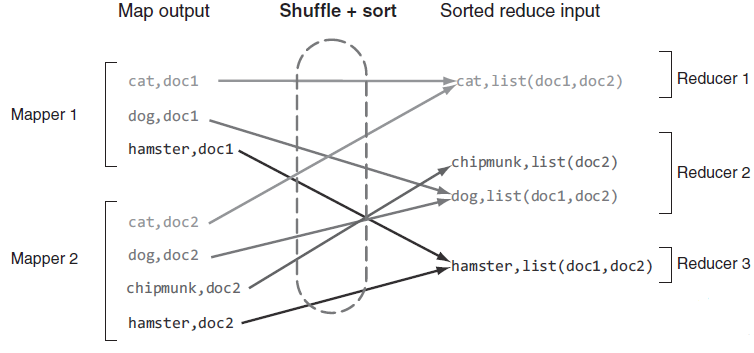
\includegraphics[width=0.75\textwidth]{images/mapreduce.png}
\caption{Etapas del \textit{framework} MapReduce, donde tenemos un problema que tiene como entrada un conjunto de archivos de texto y produce como salida por cada palabra una lista de documentos donde esa palabra haya aparecido. Imagen tomada de~\cite{Holmes12}.}
\label{mapreduce}
\end{figure*}


Tanto \texttt{map} como \texttt{reduce} se pueden definir lógicamente en función de pares clave/valor.
La función \texttt{map} produce pares clave/valor que luego son procesados por el \texttt{reduce} para producir el resultado final.
\texttt{Map} puede definirse con respecto a sus entradas y salidas de la siguiente manera:

\begin{equation*}
map(key1, value1) \rightarrow list(key2, value2)
\end{equation*}


La función toma como entrada un par con datos en cierto dominio, que representa una entrada lógica de la fuente de datos, y es aplicada en paralelo para cada uno de los pares con clave \texttt{key1}.
Por ejemplo, en el caso de un archivo, esto podría ser una línea, o en el caso de una tabla en una base de datos, podría ser una columna. 
Como resultado, de un par de entrada se produce cero o más salidas de pares clave/valor en otro dominio diferente, y con clave \texttt{key2}.
Por ejemplo, si se quiere realizar una operación de filtro, podría producirse como resultado aquellos pares que cumplen cierta condición.


Posteriormente, el \textit{framework} MapReduce se encargará de mezclar y ordenar el resultado.
Para ello, debe determinar que reductor es el encargado de recibir cada una de las salidas del \texttt{map} (proceso llamado particionamiento), y asegurar que para un reductor dado, todas las entradas se encuentra ordenadas.
El particionamiento agrupará todas las listas de aquellos pares que tengan la misma clave \texttt{key2}, y creará una sola lista para cada clave.


La función \texttt{reduce} es invocada una vez por cada clave única \texttt{key2} producida por el \texttt{map}, y cuyos valores están organizados en una lista.
\texttt{Reduce} puede definirse con respecto a sus entradas y salidas de la siguiente manera:

\begin{equation*}
reduce(key2, list(value2)) \rightarrow list(key3, value3)
\end{equation*}

Cada invocación a \texttt{reduce} produce cero o más salidas con clave \texttt{key3}, aunque típicamente se produce una sola salida.
Esta salida puede ser escrita en archivos de texto en el sistema de archivos distribuidos, producir inserciones en alguna base de datos, o ser escrito en algún repositorio de datos que dependerá del trabajo que se quiera ejecutar.


Por lo tanto, el \textit{framework} MapReduce transforma una lista clavo/valor y obtiene una lista de valores de resultado.
Esto contrasta con el uso de \texttt{map} y \texttt{reduce} en programación funcional, donde se toma una lista clave/valor y se obtiene una sola salida que combina todos los resultados obtenidos en el \texttt{map}.



\subsection{Ejemplos}

Un ejemplo del uso de MapReduce puede observarse en la Fig.~\ref{mapreduce}.
Allí cada función \texttt{map} recibe como entrada un archivo con diferentes palabras, teniendo una invocación del \texttt{map} por cada documento, y produce como salida un par \texttt{(palabra, archivo)}.
Esta salida es procesada por el módulo de mezcla y ordenamiento, el cual agrupará todas los pares que posean la misma palabra para crear un par \texttt{(palabra, lista documentos)}, que servirá como entrada para el \texttt{reduce}.
Posteriormente, se produce una invocación del \texttt{reduce} por cada par obtenido del paso anterior y se procesan.
En este caso, se podrían dejar los pares sin modificar obteniendo una lista de los documentos en los cuales aparece cada palabra.


El MapReduce también podría utilizarse para obtener la frecuencia de repetición de nombres de un listado de estudiantes.
El \texttt{map} se encargaría de generar un par \texttt{(nombre, 1)}, por cada nombre en la lista de estudiantes.
Luego, el \texttt{reduce} acumula todos los valores con el mismo nombre y emite un par \texttt{(nombre, total)}, donde \texttt{total} sería la cantidad de repeticiones de estudiantes con nombre \texttt{nombre}.



Otro ejemplo sería la obtención de un grafo de enlaces invertidos.
En este caso, la función \texttt{map} tendría como salida un par \texttt{(destino, origen)} para cada enlace a un URL \texttt{destino} encontrado en una página \texttt{fuente}.
Posteriormente, el \texttt{reduce} concatenará la lista de todos los URLs asociados a un URL \texttt{destino} específico, emitiendo un par \texttt{(destino, list(fuente))}, obteniendo todas las páginas que apuntan al URL \texttt{destino}.
Funciones como esta son muy utilizadas para el procesamiento de páginas web.


Finalmente, podemos tener otros casos en los que el \texttt{reduce} es intrascendente, como por ejemplo el ordenamiento distribuido.
Aquí el \texttt{map} extrae de cada elemento a ordenar su clave, y genera un par \texttt{(clave, elemento)}, donde el \texttt{reduce} mantiene sus pares de entrada sin cambiar.
En este caso se depende del \textit{framework} MapReduce, el cual se encarga de hacer el ordenamiento de los pares de salida del \texttt{map} antes de enviarlos al \texttt{reduce}.





\section{MapReduce para Hadoop}
\label{hadoop}


A partir de la propuesta de implementación de Google~\cite{MapReduce04}, diversas implementaciones del modelo de programación MapReduce han surgido, donde una de las más conocidas es la implementación de Hadoop.
En Hadoop se tiene un motor MapReduce que corre encima del sistema de archivos HDFS (ver Fig.~\ref{motor}), el cual está implementado en Java.
Sus elementos principales son: Job Client,  Job Tracker, Task Tracker, y Child.


\begin{figure*}[htbp!]
\centering
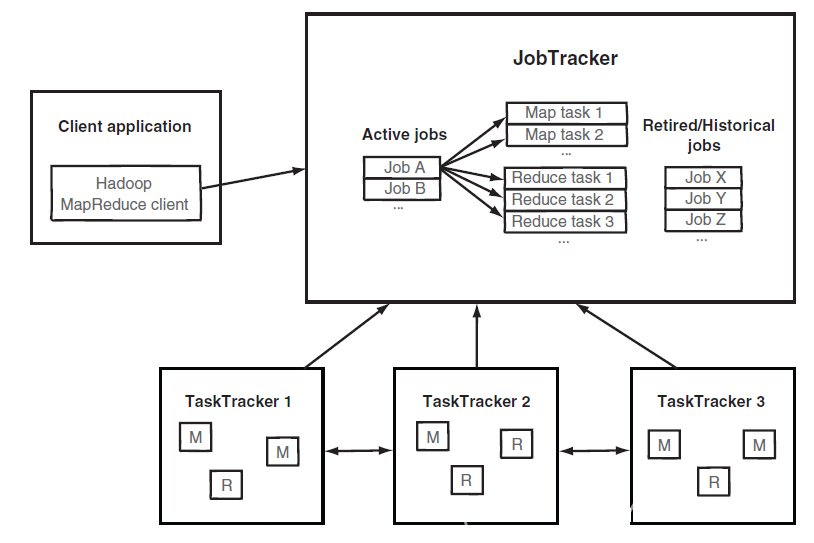
\includegraphics[width=0.7\textwidth]{images/motor.png}
\caption{Motor MapReduce de Hadoop. Imagen tomada de~\cite{Holmes12}.}
\label{motor}
\end{figure*}
	


Un trabajo o \textit{job} MapReduce a ejecutar consiste en una función \texttt{map} y una función \texttt{reduce}, las cuales indica el usuario al Job Client para comenzar la ejecución del trabajo.
El Job Client se encarga de validar la configuración, generar la partición de la data, generar las copias de los recursos necesarios por el Job Tracker y Task Tracker, y entregar el trabajo al Job Tracker.


El Job Tracker se encarga de coordinar las actividades para enviar trabajos a los nodos esclavos Task Tracker en el cluster, dividiendo el trabajo en tareas \texttt{map} y \texttt{reduce}.
Además, contiene funciones de recuperación de tareas en caso de fallos y de rastreo del estatus del trabajo. 
Cuando el Job Tracker se prepara parar correr un trabajo, primero obtiene la información dividida en el área compartida donde el Job Client colocó la información, crea una tarea \texttt{map} por cada división y asigna cada tarea \texttt{map} a un Task Tracker.
Cada una de estas son conocidas como Child.
Cuando las tareas \texttt{map} finalizan y los resultados están disponibles, el Job Tracker se encarga de crear tareas \texttt{reduce}, asignar a la tarea sus correspondientes resultados de cada \texttt{map}, y asigna cada tarea a un Task Tracker.
Se considera que un trabajo está completado cuando todas las tareas \texttt{map} y \texttt{reduce} son completadas.


Debido a que el sistema de archivos de Hadoop permite tener conocimiento de donde se encuentran los datos, el Job Tracker tratará de ejecutar tratando de mantener los datos lo más cercano posible, procurando de ejecutar los trabajos en el nodo donde se encuentra la información.
Si esto no es posible, se seleccionará un nodo que se encuentre cercano (en el mismo rack de ser posible), reduciendo el uso de tráfico de datos.


Por otro lado, el Task Tracker es un proceso demonio que se encarga de producir procesos hijos para ejecutar la operación \texttt{map} o \texttt{reduce}, y reportar el estatus de los mismos al Job Tracker.
Típicamente, las tareas \texttt{map} leen las entradas desde el HDFS, y escriben las salidas al disco local. 
En cambio las tareas \texttt{reduce} leen las salidas del \texttt{map} desde la red y escriben sus salidas al HDFS.



Por cada proceso que el Task Tracker tenga que ejecutar, se crea una máquina virtual de Java para prevenir que un error en este proceso termine la ejecución del Task Tracker.
Cada Task Tracker tiene un número disponible de espacios.
El Job Tracker asigna trabajos al espacio disponible que esté más cerca de los datos.
Además, cada cierto tiempo el Task Tracker envía una señal al Job Tracker para indicarle su estatus. 
En caso de que un Task Tracker falle, el Job Tracker se encargará de volver a programar el trabajo fallido.
Si un Task Tracker es muy lento podría retrasar todo el trabajo del MapReduce, especialmente cerca del final, donde se podría terminar esperando por la tarea más lenta.




\subsection{YARN}

Posteriormente, Hadoop adoptó YARN~\cite{Yarn13} (Yet Another Resource Negotiator), cuya funcionalidad is permitir al sistema servir como un \textit{framework} de procesamiento de datos generales.
De esta manera, soporta otros modelos de programación aparte del MapReduce, mejorando la escalabilidad y la utilización de recursos, sin realizar cambios en el HDFS o el modelo de programación.
YARN apunta a eliminar los cuellos de botella de la arquitectura maestro/esclavo.


Con YARN, las responsabilidades del Job Tracker son divididas en dos procesos diferentes: el Resource Manager y el Application Master.
El Resource Manger se encarga del manejo dinámico de los recursos, utilizando la noción de \textit{containers}, en vez de los espacios \texttt{map}/\texttt{reduce} estáticos presentes en los Task Tracker.
Los \textit{containers} son configurados basados en la información correspondiente a la memoria disponible, CPU y la capacidad de disco.
También posee un planificador añadible, el cual puede utilizar diferentes estrategias para asignar actividades a los nodos disponibles.

El Application Master es un proceso específico del \textit{framework}, permitiendo que otros modelos de programación puedan ser ejecutados sobre YARN.
Se encarga de negociar recursos con el Resource Manager y supervisar las tareas ya programadas.







\section{Limitaciones}
\label{limits}

A pesar de las bondades presentadas por MapReduce, el modelo de programación tiene algunas desventajas y limitaciones que vale la pena mencionar.
MapReduce no garantiza ser rápido, por lo que no es factible su uso para aplicaciones en tiempo real.
Además, a pesar de que el programador solo debe de preocuparse de implementar las funciones \texttt{map} y \texttt{reduce}, la operación de mezclado y ordenamiento puede ser costosa, por lo que el programador debe tomarlas en cuenta.
Especialmente si el \texttt{map} produce una gran cantidad de datos de salida, esta etapa puede verse comprometida, teniendo un gran impacto en el desempeño y la escalabilidad.


Al ser MapReduce un modelo de programación que no comparte información entre las ejecuciones, hace que programas que necesiten sincronización global, mantener estado o compartir los datos sean difíciles de implementar.
Además, el MapReduce no se adapta de manera fácil a algoritmos que necesiten iterar varias veces, o que sean aplicaciones interactivas.
Esto se debe a que este modelo está optimizado para trabajar por lotes, con datos ya presentes a priori.


Por último, cuando se diseña un algoritmo MapReduce, el programador debe en cuenta el costo asociado a la comunicación de los datos entre los diferentes nodos del sistema. 
En ocasiones el costo de la comunicación domina el costo de la computación, por lo que otro tipo de modelos de programación podrían ser más beneficiosos.


\section{Conclusiones}
\label{conclu}

En este trabajo se realizó una introducción teórica al modelo de programación MapReduce y su implementación en Hadoop, siendo esta una de las herramientas más utilizadas en la actualidad para la ciencia de datos, mostrando algunos ejemplos teóricos de problemas que pueden resolverse con este modelo.
Como pudo observarse el modelo es simple, y soporta de manera efectiva el paralelismo.
Por ello, el programador puede abstraerse de problemas inherentes a la programación paralela y distribuida debido a que las implementaciones MapReduce se encargan del balanceo de cargas, eficiente uso de la red, tolerancia a fallas, entre otros.


También se expusieron algunas limitaciones presentes en el modelo, mostrando que hay todavía diversos problemas a resolver y optimizaciones a considerar.
Sin embargo, el desarrollo de estas optimizaciones es un gran desafío, debido a la necesidad de mantener todas las ventajas que posee este modelo de programación, demostrando que sistemas para Big Data y especialmente para MapReduce siguen siendo un área de investigación abierto.



\balance
\bibliographystyle{IEEEtran}
\bibliography{books}



\end{document}



